\documentclass{beamer}

\usetheme{Berlin}
\usepackage{hyperref}
\usepackage{graphicx}


\title{Middle Term Presentation}

\author{Mingkun Yang \\
\texttt{minyan09@student.hh.se}}

\institute{
Halmstad University\\
}
\date{}

\AtBeginSection[]
{
\begin{frame}<beamer>{Outline}
	\tableofcontents[currentsection]
\end{frame}
}

\begin{document}

\begin{frame}
	\titlepage
\end{frame}

\begin{frame}{Outline}
	\tableofcontents[pausesections]
\end{frame}

\section{Review}
\begin{frame}{Project reviewing}
	\begin{itemize}
		\item
			Objective
			\pause
		\item
			Concepts
			\begin{itemize}
				\item
					Question(Sharable Content Object)
					\pause
				\item
					Test(Package)
			\end{itemize}
	\end{itemize}

\end{frame}

\section{Finished tasks}
\begin{frame}{tasks}
	\begin{itemize}
		\item
			Import whole test
			\pause
		\item
			Import single question
	\end{itemize}
\end{frame}

\section{Unfinished tasks}
\begin{frame}{Packaging}
	\begin{itemize}
		\item
			Organize the report
			\pause
		\item
			Construct one package
	\end{itemize}
\end{frame}

\section{Original plan}
\begin{frame}{Gantt Chart}
	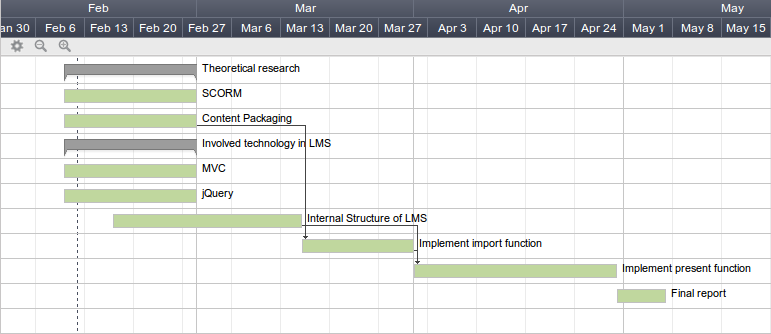
\includegraphics[scale=0.4]{Ganttold.png}
\end{frame}

\section{Revised plan}
\begin{frame}{Gantt Chart}
	\hspace*{-5mm}
	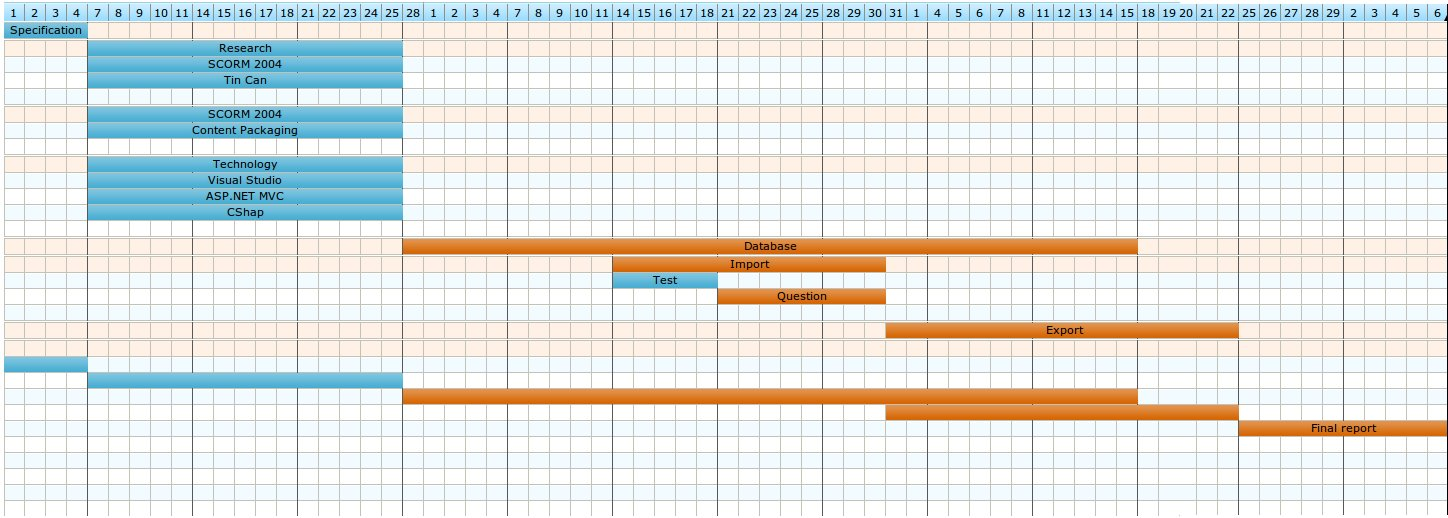
\includegraphics[width=120mm, height=60mm]{Ganttnew.jpg}
\end{frame}

\end{document}
